\subsection{Longitudinal Time-Function Sensitivity Analysis}

Treatment time was measured in months for clinical interpretation and converted to years in the Bayesian likelihood. The primary fitted joint model used a parsimonious nonlinear time trend,
\[
f_{\log}(x)=\beta_1\log(1+x)+\beta_2\{\log(1+x)\}^2,
\]
where \(x\) denotes years since treatment initiation. This specification was chosen for the primary fitted analysis because it captures rapid early molecular decline followed by later flattening while preserving a small number of time-effect parameters in a cohort of 87 patients.

To assess whether the longitudinal trajectory required greater flexibility, we compared three candidate population time functions in a screening mixed-model analysis: the current log-quadratic function, a clinically knotted piecewise-linear function, and a low-rank spline proxy. The piecewise-linear model used knots at 3, 6, 12, 24, and 60 months, corresponding to clinically meaningful monitoring periods. The spline proxy used four degrees of freedom for the population time trend. In all screening models, patient-level heterogeneity was represented by a random intercept and a single random time slope. Because this screening step was designed to evaluate time-function shape rather than replace the Bayesian joint model, assay-floor observations were treated as observed at \(-5.0\); final inference should therefore be based on a full Bayesian refit using the left-censoring likelihood for floor observations.

For a renewed Bayesian model, the general longitudinal trajectory can be written as
\[
\eta_i(x_{ij}) =
\beta_0+f(x_{ij})+\beta_{\mathrm{BM}}I(\mathrm{bone\ marrow}_{ij})
+b_{0i}+b_{1i}\log(1+x_{ij}),
\]
where \(f(x)\) is selected from the candidate time functions. A low-rank penalized spline may be specified as
\[
f_{\mathrm{S}}(x)=\sum_{k=1}^{K}\theta_k B_k(x),
\qquad
\theta_k-2\theta_{k-1}+\theta_{k-2}\sim N(0,\sigma_f^2),
\]
with \(K\) kept small and \(\sigma_f\) assigned a shrinkage prior. A soft monotone-decline sensitivity analysis can be added by penalizing positive increments in the population curve over an ordered time grid,
\[
\log p_{\mathrm{mono}} \propto
-\frac{1}{2\sigma_{\mathrm{mono}}^2}
\sum_{g=2}^{G}\left[\max\{0,f(x_g)-f(x_{g-1})\}\right]^2.
\]
This regularization discourages biologically implausible late population-level rebound while still allowing patient-specific increases through the random effects and measurement model.

\begin{table}[!htbp]
\centering
\caption{Screening comparison of longitudinal time functions. This table is an approximate mixed-model benchmark for time-function selection; floor observations are treated as observed at \(-5.0\) and final inference should be based on the Bayesian joint model with censoring.}
\label{tab:time-function-comparison}
\resizebox{\linewidth}{!}{%
\begin{tabular}{lrrrrrrr}
\toprule
Time function & Time parameters & AIC & Non-floor RMSE & Interval Brier & Interval calibration slope & Patient Brier & Patient calibration slope \\
\midrule
Log-quadratic in log(1+t) & 2 & 1726.9 & 1.095 & 0.123 & 1.00 & 0.179 & 1.62 \\
Piecewise linear knots 3, 6, 12, 24, 60 months & 6 & 1735.0 & 1.134 & 0.123 & 1.00 & 0.179 & 1.47 \\
Low-rank spline proxy (4 df) & 4 & 1723.4 & 1.102 & 0.127 & 1.00 & 0.187 & 1.41 \\
Soft monotone-decline constrained spline & 4 & -- & -- & -- & -- & -- & -- \\
\bottomrule
\end{tabular}
}%
\end{table}



\begin{figure}[!htbp]
\centering
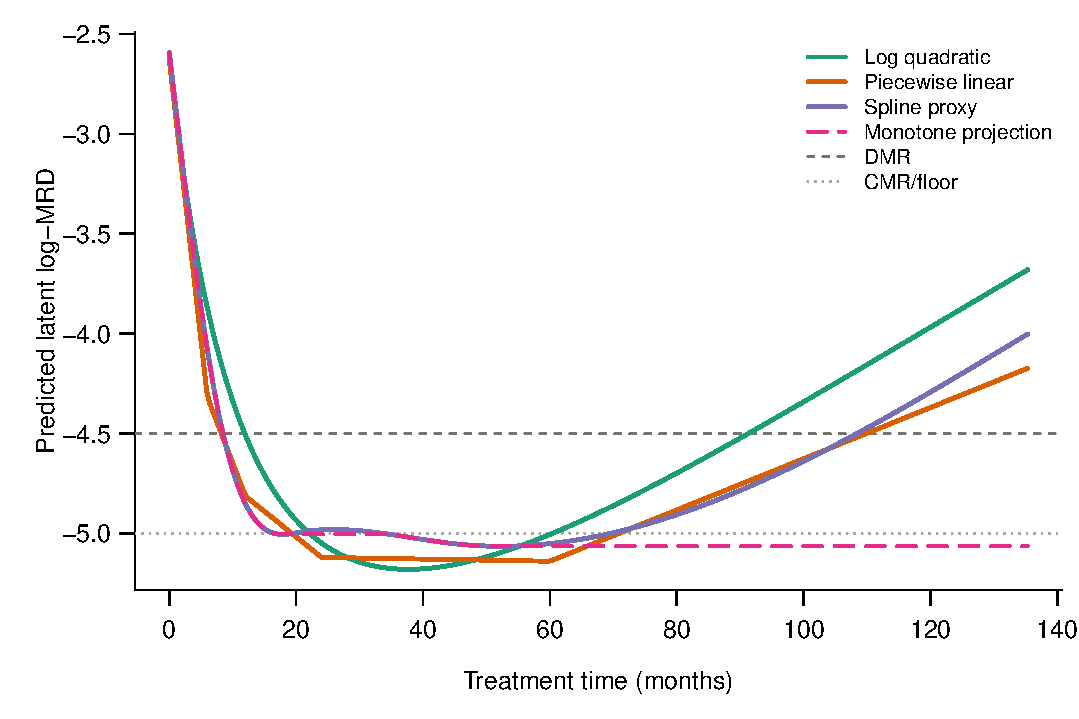
\includegraphics[width=0.92\linewidth]{figure_12_time_function_population_trends.pdf}
\caption{Screening comparison of population time trends for log-MRD. Knots for the piecewise-linear model were specified at 3, 6, 12, 24, and 60 months. The monotone curve is a soft population-level projection of the spline trend and is shown as a biological sensitivity target rather than a replacement for patient-level variation. DMR and CMR/floor thresholds are shown at log-MRD \(-4.5\) and \(-5.0\), respectively.}
\label{fig:time-function-trends}
\end{figure}

In the screening comparison, the low-rank spline proxy had the lowest AIC (1723.4), indicating modest improvement in apparent longitudinal fit relative to the current log-quadratic model (AIC 1726.9) and the piecewise-linear model (AIC 1735.0). However, the current log-quadratic model had the lowest non-floor RMSE (1.095) and the lowest patient-level Brier score in the two-stage calibration proxy (0.179). The piecewise-linear model had a similar interval-level Brier score (0.123) but required six fixed time parameters, increasing overfitting risk in this cohort. The spline proxy did not improve the calibration proxy, with interval-level Brier score 0.127 and patient-level Brier score 0.187.

These results support a conservative interpretation. The current log-quadratic function remains a defensible primary specification for the fitted model because it is parsimonious, stable, and already demonstrated acceptable HMC diagnostics in the full Bayesian analysis. If the model is renewed to allow a more flexible longitudinal trajectory, the preferred candidate is a low-rank penalized spline with independent patient-level random intercept and random log-time slope, combined with a soft population-level monotone-decline sensitivity analysis. Such a renewed model should be adopted as primary only after a full Bayesian refit confirms acceptable convergence, posterior predictive performance, floor-probability calibration, and interval- and patient-level DMR calibration.
